%File: formatting-instruction.tex
\documentclass[letterpaper]{article}
\usepackage{aaai}
\usepackage{times}
\usepackage{helvet}
\usepackage{courier}
\usepackage{graphicx}
\usepackage{csvsimple}
\frenchspacing
\nocopyright
\setlength{\pdfpagewidth}{8.5in}
\setlength{\pdfpageheight}{11in}
\pdfinfo{
/Title (Insert Your Title Here)
/Author (Put All Your Authors Here, Separated by Commas)}
\setcounter{secnumdepth}{0}
\graphicspath{ {./picture/} }
 \begin{document}
% The file aaai.sty is the style file for AAAI Press
% proceedings, working notes, and technical reports.
%
\title{}
\author{}
\maketitle
\begin{abstract}
\begin{quote}
\end{quote}
\end{abstract}

\section{Data Source}

The amount of pollutants observed in each station is provided by Yang Yu. The shape of China and all provinces can be found on GADM\footnote{https://gadm.org/index.html}. 

\section{Interpolation}

There are many multivariate interpolation method for 2D interpolation, such as bilinear, bicubic methods (wiki). However, when applying these methods, there are always some empty parts in the map. It is because these methods are used to interpolate regular grid, but the position of stations does not form a regular grid. For this sort of scattered data, radial basis function(RBF) is used for interpolation in the paper (wiki). The function form is rather simple. For any point $\mathbf{x}$, 
\begin{eqnarray}
  y(\mathbf{x}) = \sum_{i=1}^Nw_i\phi\left(\|\mathbf{x} - \mathbf{x_i}\|\right). 
\end{eqnarray}
$\mathbf{x_i}$ are those observation points and $\phi$ is a customized function. The estimation of $w_i$ can be solved by linear least square.

Below several different functions are tested respectively. 
\begin{figure}[h]
  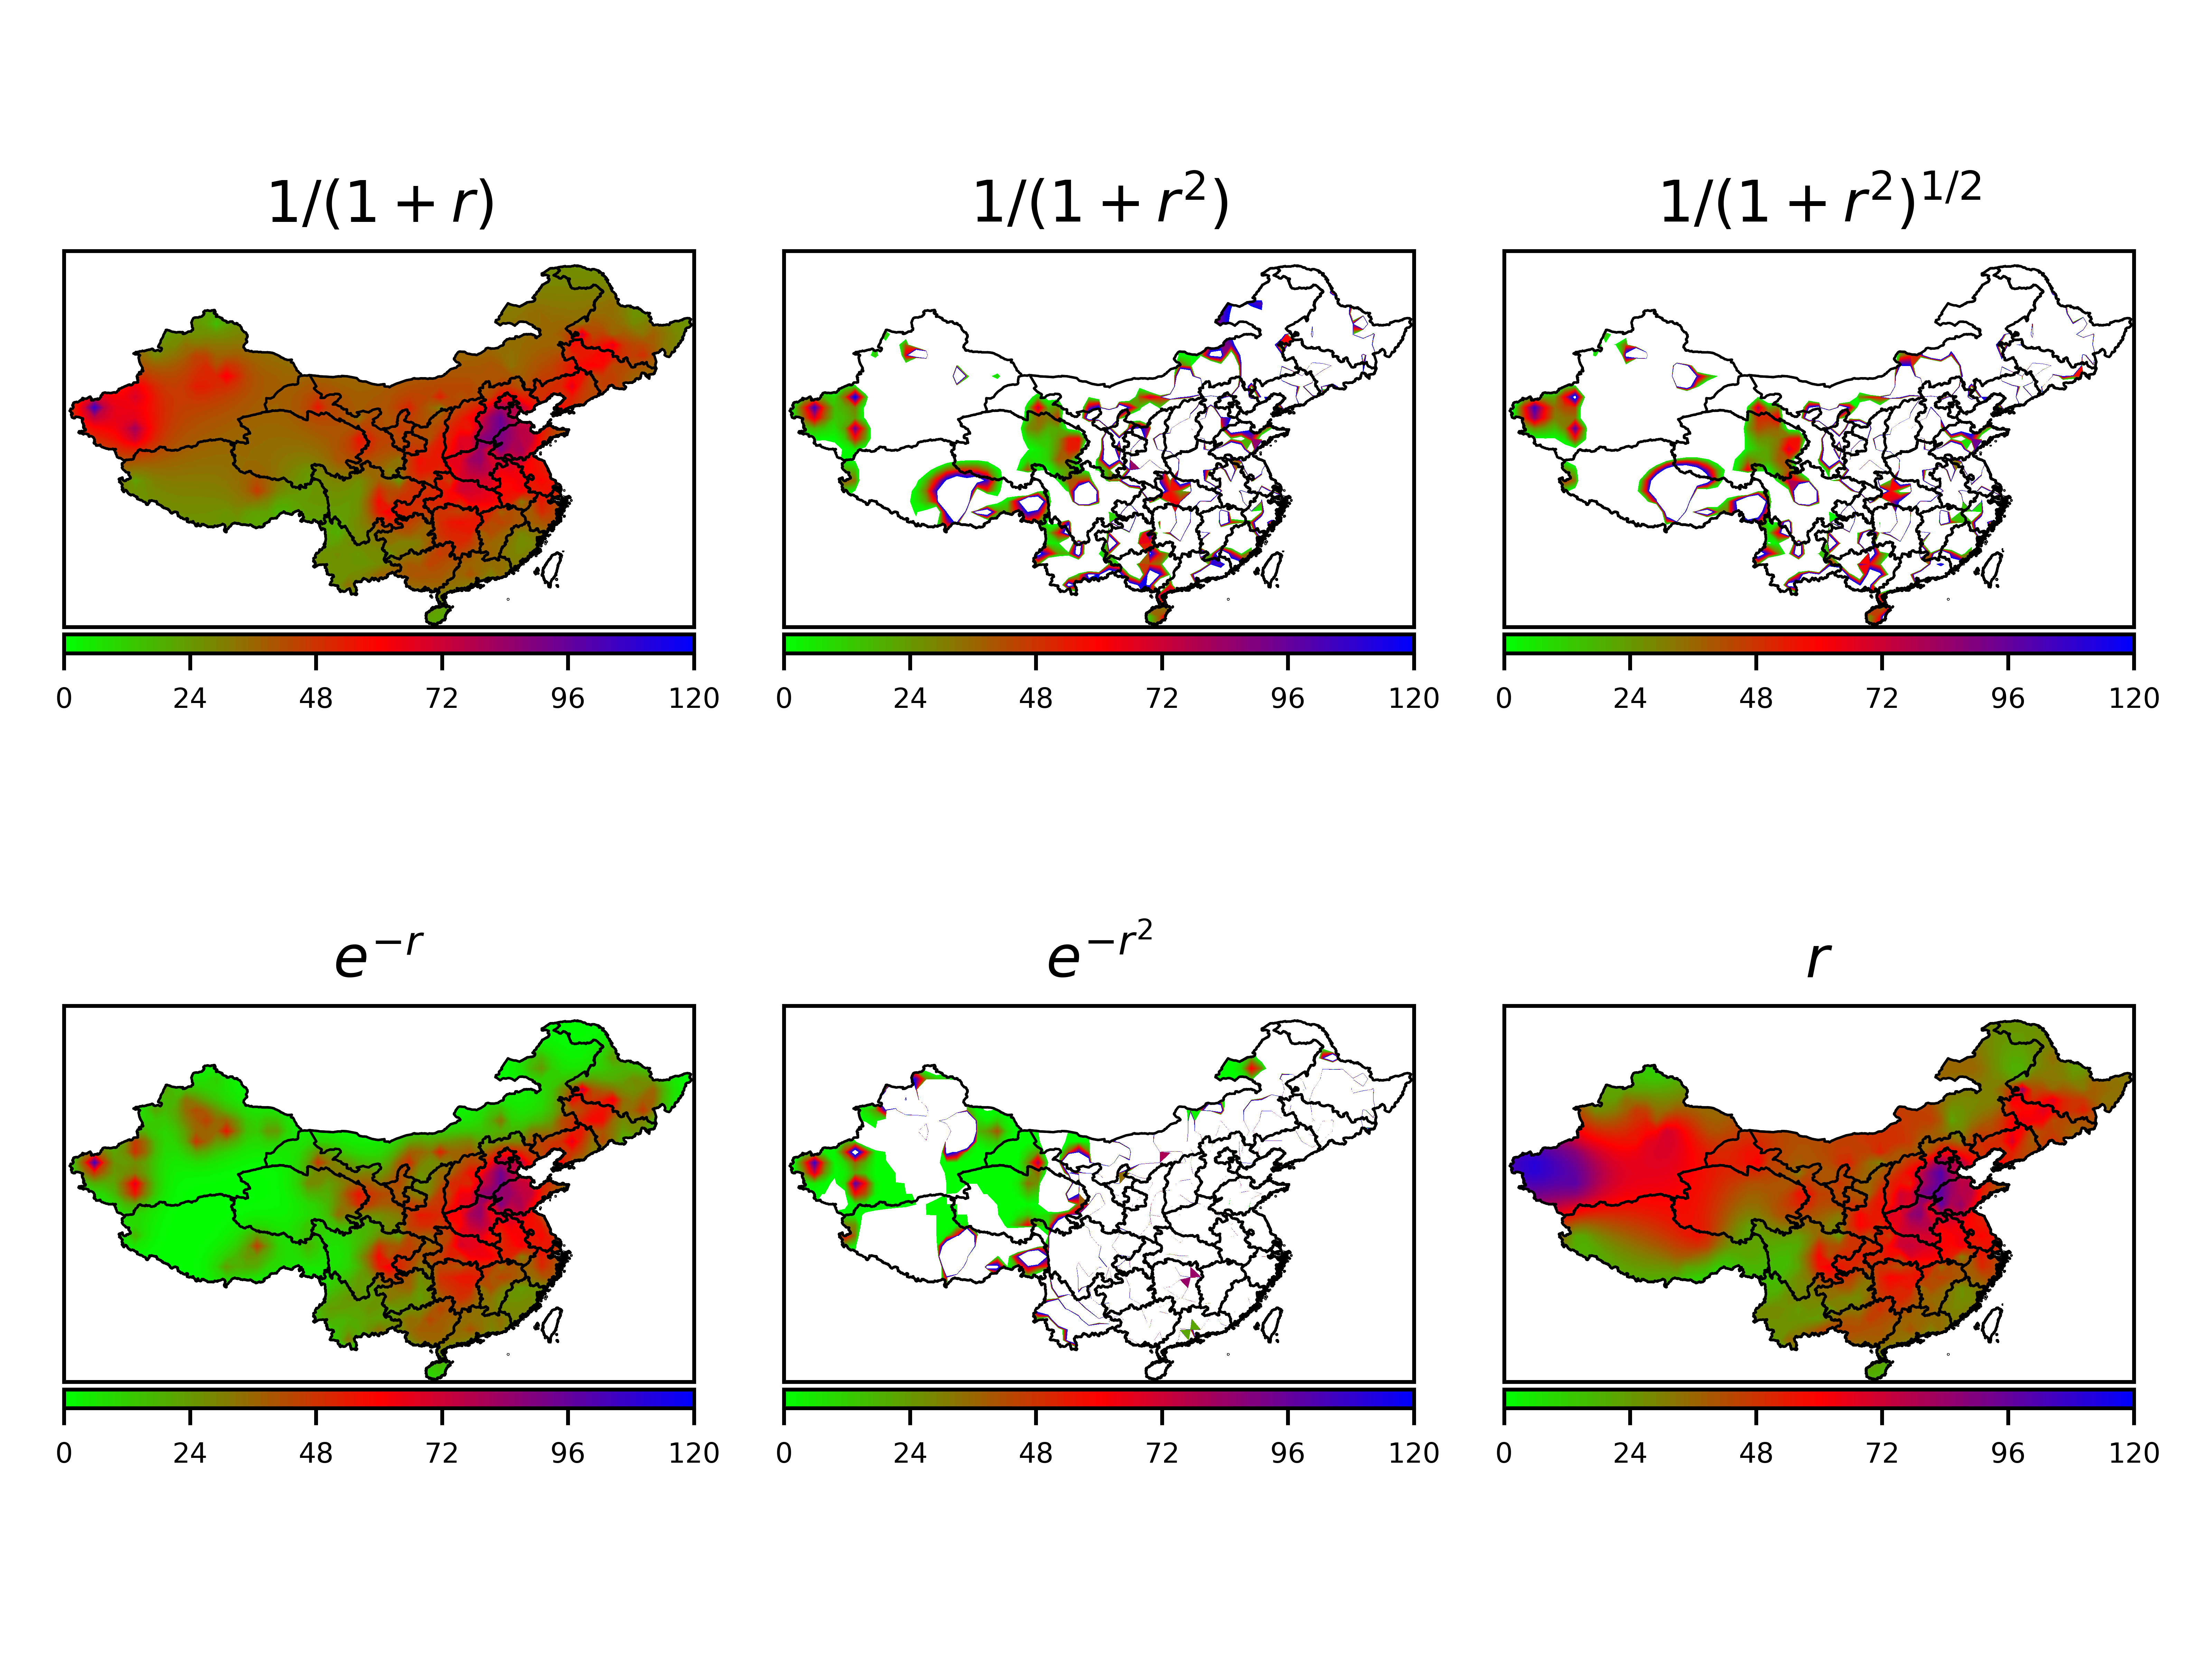
\includegraphics[width = 8.5cm]{Interpolation_from_20150102_to_20151231.png}
  \caption{Interpolation of annually average concentration of PM2.5 using different
    $\phi(r)$}
  \label{figure:0}
  \centering
\end{figure}

In these images, those interpolated by ``quadratic'' methods have a lot of empty parts caused by negative value. However, this does not happen in ``linear'' methods. When comparing ``linear'' methods $1/(1+r), e^{-r}, r$, the images in Xinjiang are quite different. In $e^{-r}$, concentration degrades so rapidly that only points close to observation station are not green. In contrast to $e^{-r}$, $r$-interpolation degrades much slower and most of Xinjiang is red. $1/(1+r)$ is the intermediate between $e^{-r}$ and $r$. Due to lack of data, we cannot determine which function is the best. For simplicity, $r$-interpolation is used throughout the project. 

 One of the advantage of RBF is that $y$ is linear. Therefore, when it needs to compute the average value interpolation, calculating interpolation in each hour and then taking average for each point are not necessary. We can directly compute the average value for each station and then calculate the interpolation, which saves much of the time.

\section{Space Distribution}

The high accuracy distributions in China of PM$_{2.5}$, PM$_{10}$, SO$_{2}$, NO$_{2}$, O$_{3}$, and CO, which are the main air pollutants, are got by the data and interpolation method mentioned above. The regularities of space distributions of these air pollutants are summarized in this part.
\begin{figure}[h]
  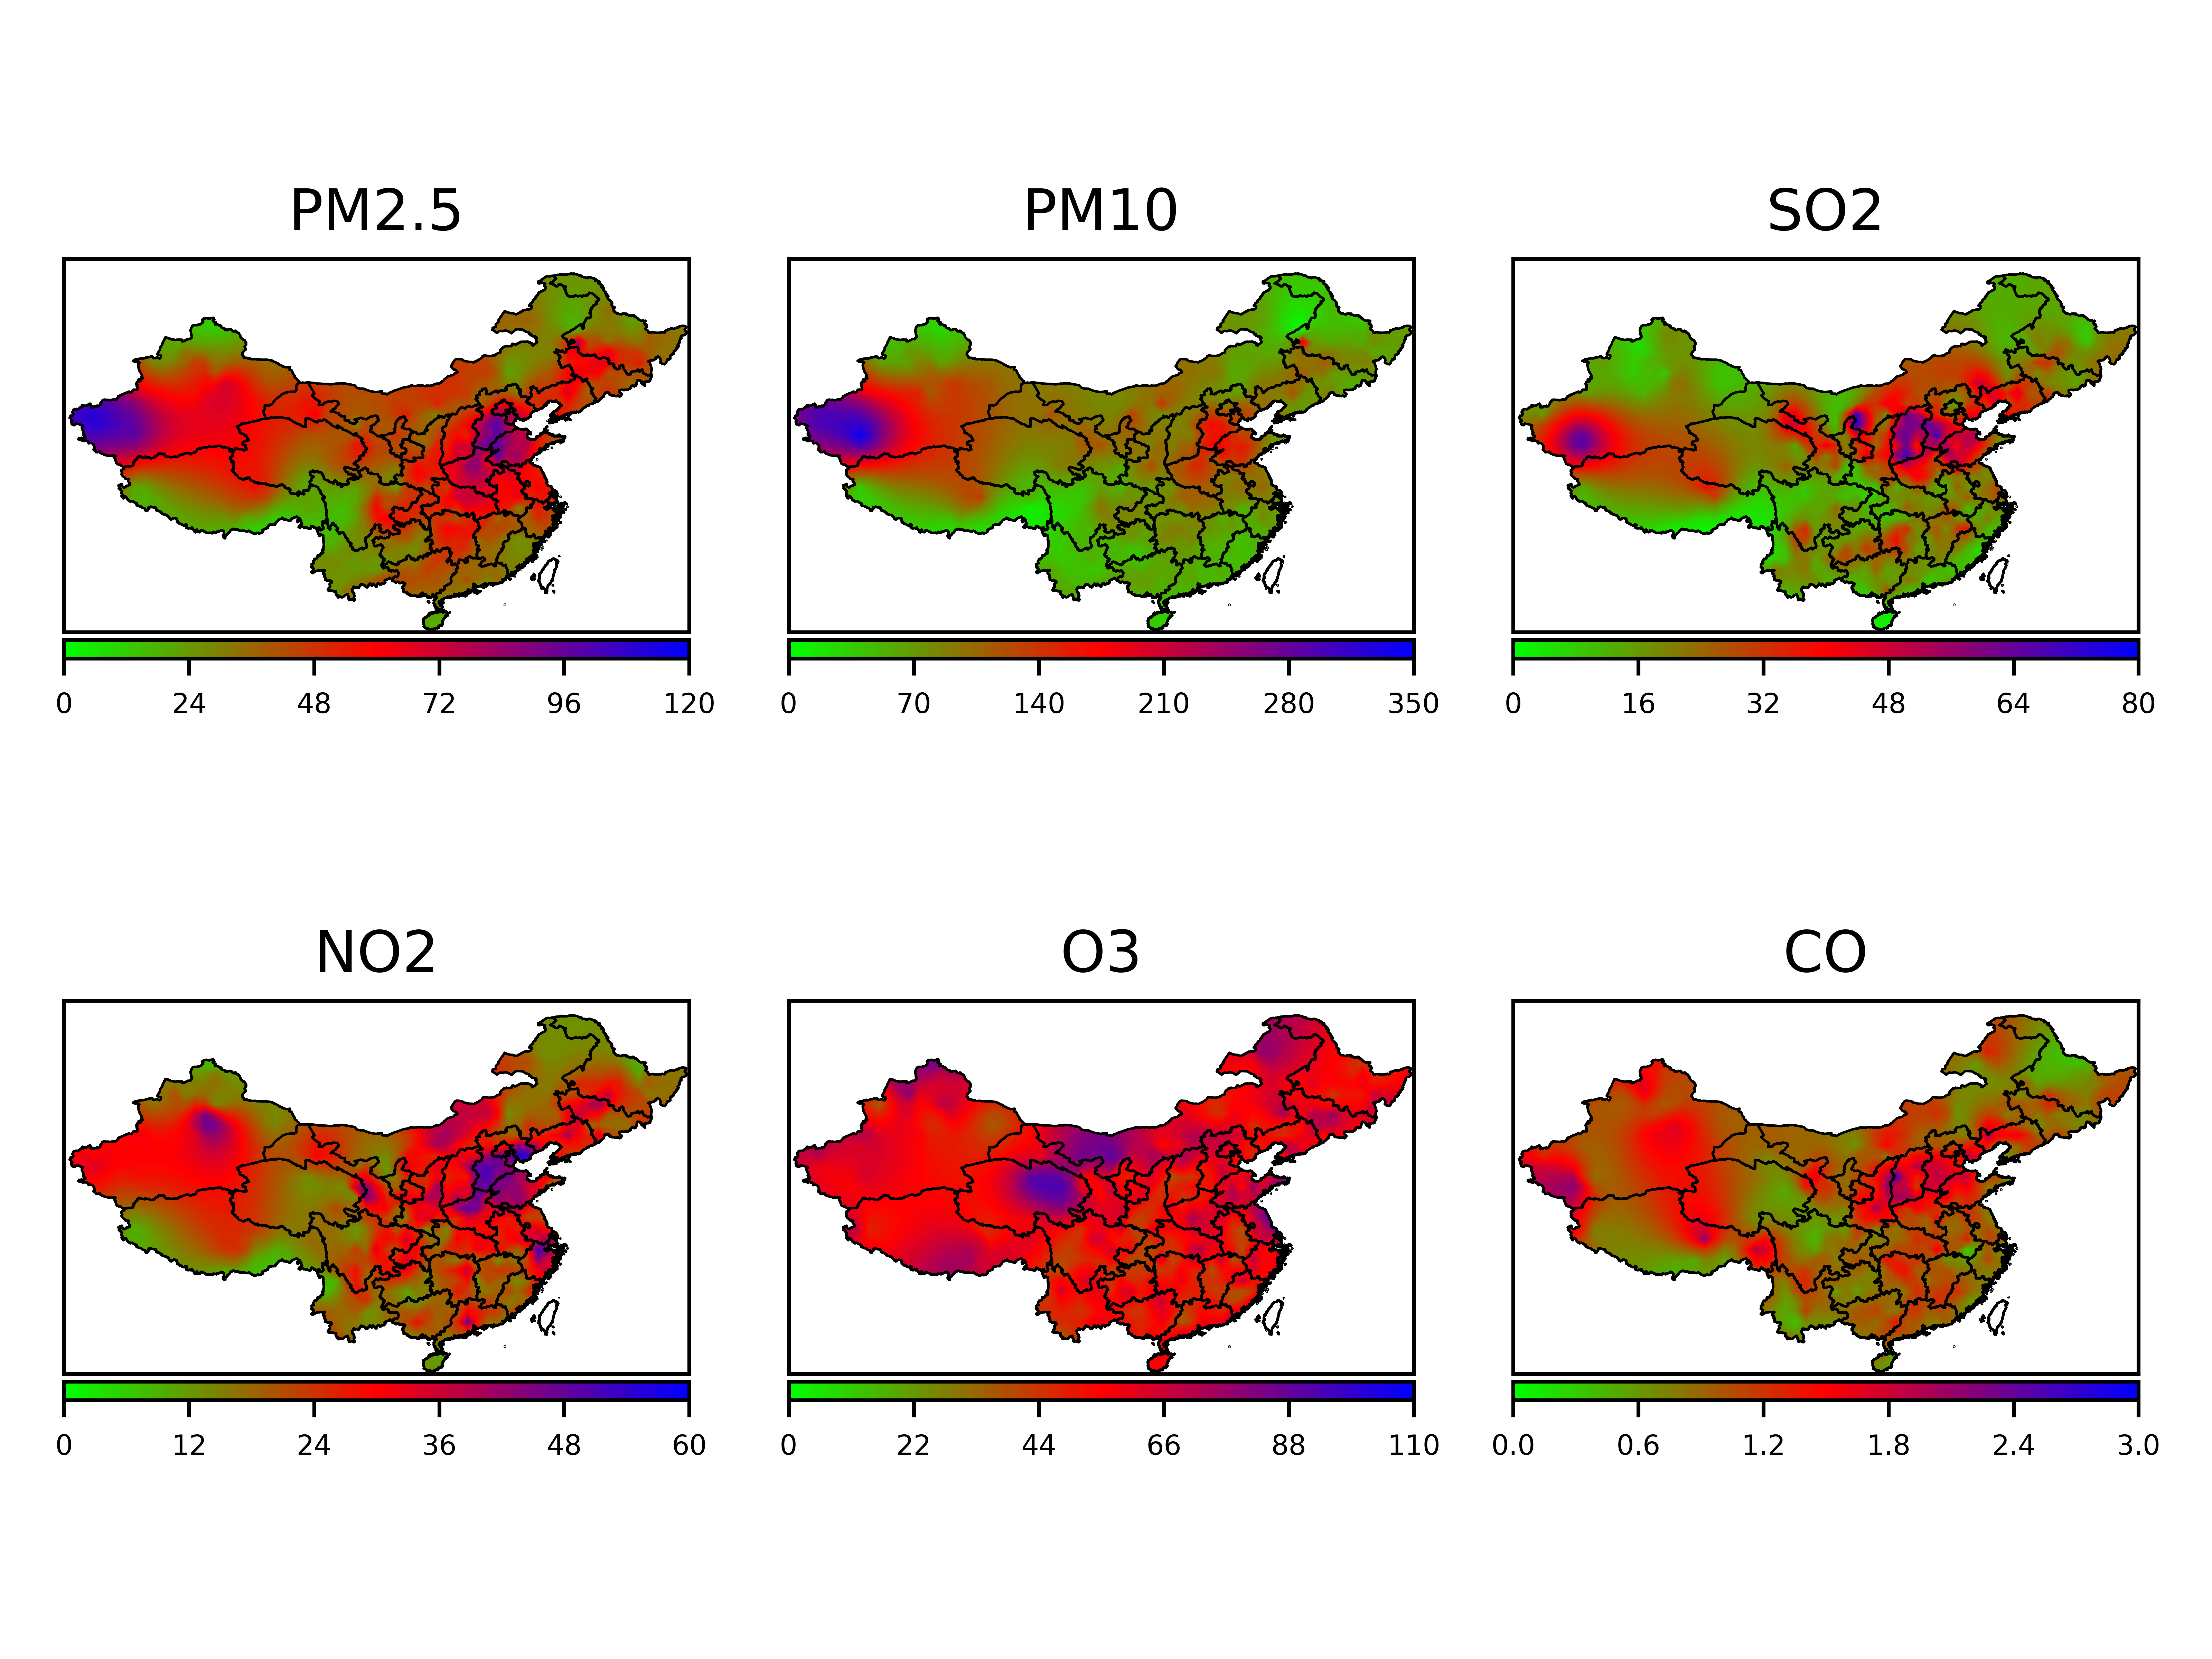
\includegraphics[width = 8.5cm]{Interpolation_from_20150102_to_20151231_linear.png}
  \caption{Distribution of annually average concentration of pollutants}
  \label{figure:1}
  \centering
\end{figure}

By an overview of these figures, a general impression of the air quality over China can be got.

In the figures which represent PM$_{2.5}$, PM$_{10}$, SO$_{2}$, NO$_{2}$, and CO, there are two areas which are in the south of Xinjiang and around Hebei with the most serious pollution, which are the blue areas in the figures. The distribution of the red areas, which are the areas with pollution not so serious, is radial from these two points. In the south of China and the northeast of China, the pollution is slight in comparison.

It is special for the figure which represent O$_{3}$. It shows that the distribution is average and that the area with the maximum concentration of O$_{3}$ is around the northeast of Qinghai, the middle of Shaanxi and the west of Inner Mongolia.

\begin{table*}
  \begin{tabular}{c|cccccc}
    \bf{Region} & \bf{PM2.5} & \bf{PM10} & \bf{SO2} & \bf{NO2} & \bf{O3} & \bf{CO} \\\hline
    \csvreader[head to column names]{./csv/regional_annual_pollutant.csv}{}{\\\csvcoli & \csvcolii & \csvcoliii & \csvcoliv & \csvcolv & \csvcolvi & \csvcolvii}
  \end{tabular}
  \centering
  \caption{Annually average concentration of pollutants in seven regions}
  \label{table:1}
\end{table*}

In the sheet, the pollutants are considered in seven main regions of China, which are Central China, North China, South China, East China, Northeast, Northwest, and Southwest. The sheet shows the annual average concentrations of different pollutants in different regions, which is calculated by the result of interpolation method. In keeping with the overview, the annual average concentrations of all pollutants in Northwest, South China, and Southwest are obviously smaller than those in Central China, North China, East China, and Northwest.

As it is mentioned above, the two regions with the most serious pollution in China are in Xinjiang and around Hebei. However, the factors that make the high pollution are not the same for these two regions. The heavy industry with high emission in Hebei, such as iron and steel industry and cement industry, is one of the factors that make the poor air quality. However, the factors in Xinjiang are most natural factors but not man-made, such as climate and physiognomy. For example, the desert and sand storm will increase the concentration of particulate matter a lot.

There is something that should be explained. Because of the maldistribution of the observation points, the estimation by interpolation in some regions, such as in the west of China and Inner Mongolia, may be different with the fact. The whole Inner Mongolia is considered in the North China. As a result, it is not strange to see that the pollution in North China is not so serious, although the pollution in Beijing-Tianjin-Hebei Region is the most serious as we know.

\section{Time Distribution}

The data also shows some regularities of the time distribution of pollutants. In this part, the regularities will be analysed in one day, in a week, and in the whole year. That is because human activities, such as work and rest, changes in one day cycle, in one week cycle, and in one year cycle. In the whole year, the climatic conditions change with the seasons, which may be the factors that affect pollutants concentration. Thus, it is a reasonable guess that the concentration of pollutants will have the certain regularity in one day, in one week, and in the whole year.

x\begin{figure}[h]
  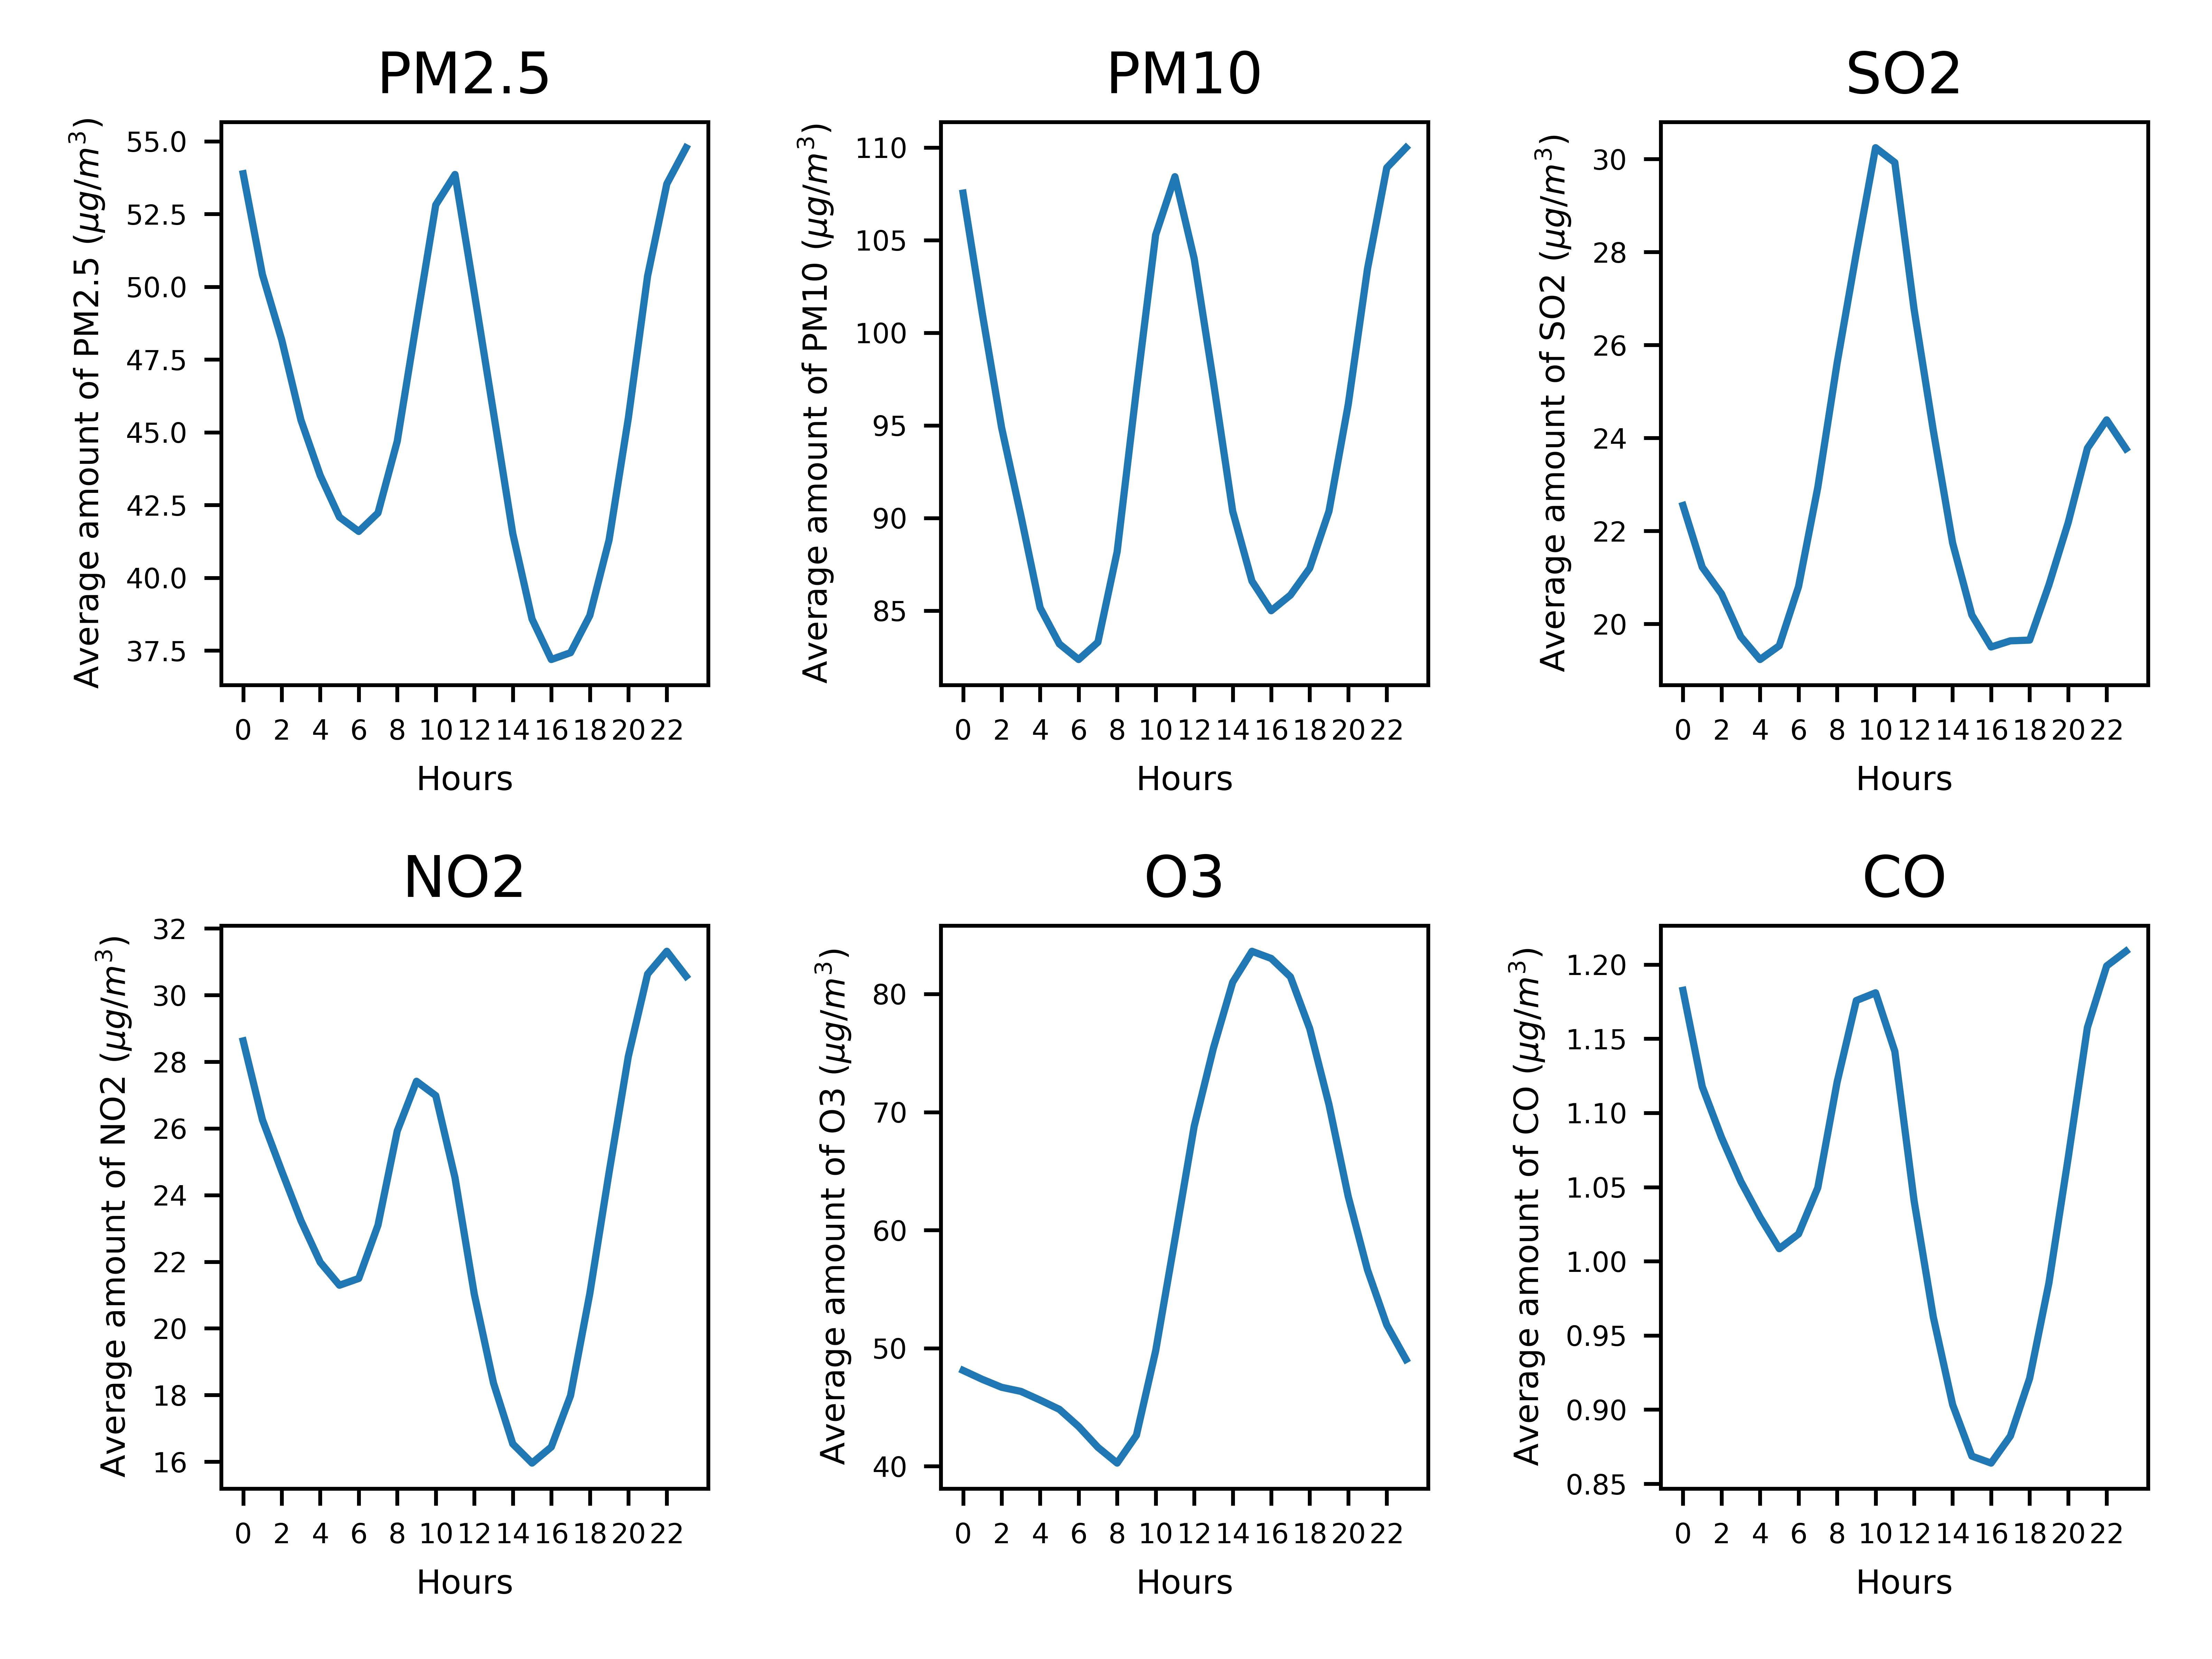
\includegraphics[width = 8.5cm]{dailyavg_pltn.png}
  \caption{Daily average concentration of pollutants}
  \label{figure:2}
\end{figure}

The figures shows the change curves of average concentration over 24 hours for different pollutants. The curves of PM$_{2.5}$, PM$_{10}$, CO, and NO$_{2}$ are similar, which have two peaks with similar height. one peak appears around 10h, and the other peak appears around 22h. The curve of SO$_{2}$ also has two peaks, but the peak appears around 22h is much lower than the other. The curve of O$_{3}$ is special, which only has one peaks that is around 15h.

According to some previous researches (yuyang), human daily activity is a factor of the regularity. The peak around 10h, which is time for trips, appears because of the traffic. The concentration increases at afternoon because of human activities after work, such as traffic and cooking. The concentration reaches another peak around 22h because the industrial production at night. The curve of O$_{3}$ seems strange, because being different with other pollutants, it is produced at high temperature from volatile organic compound and oxynitride. Thus its curve reaches the peak around 3h, when the temperature is highest.

\begin{figure}[h]
  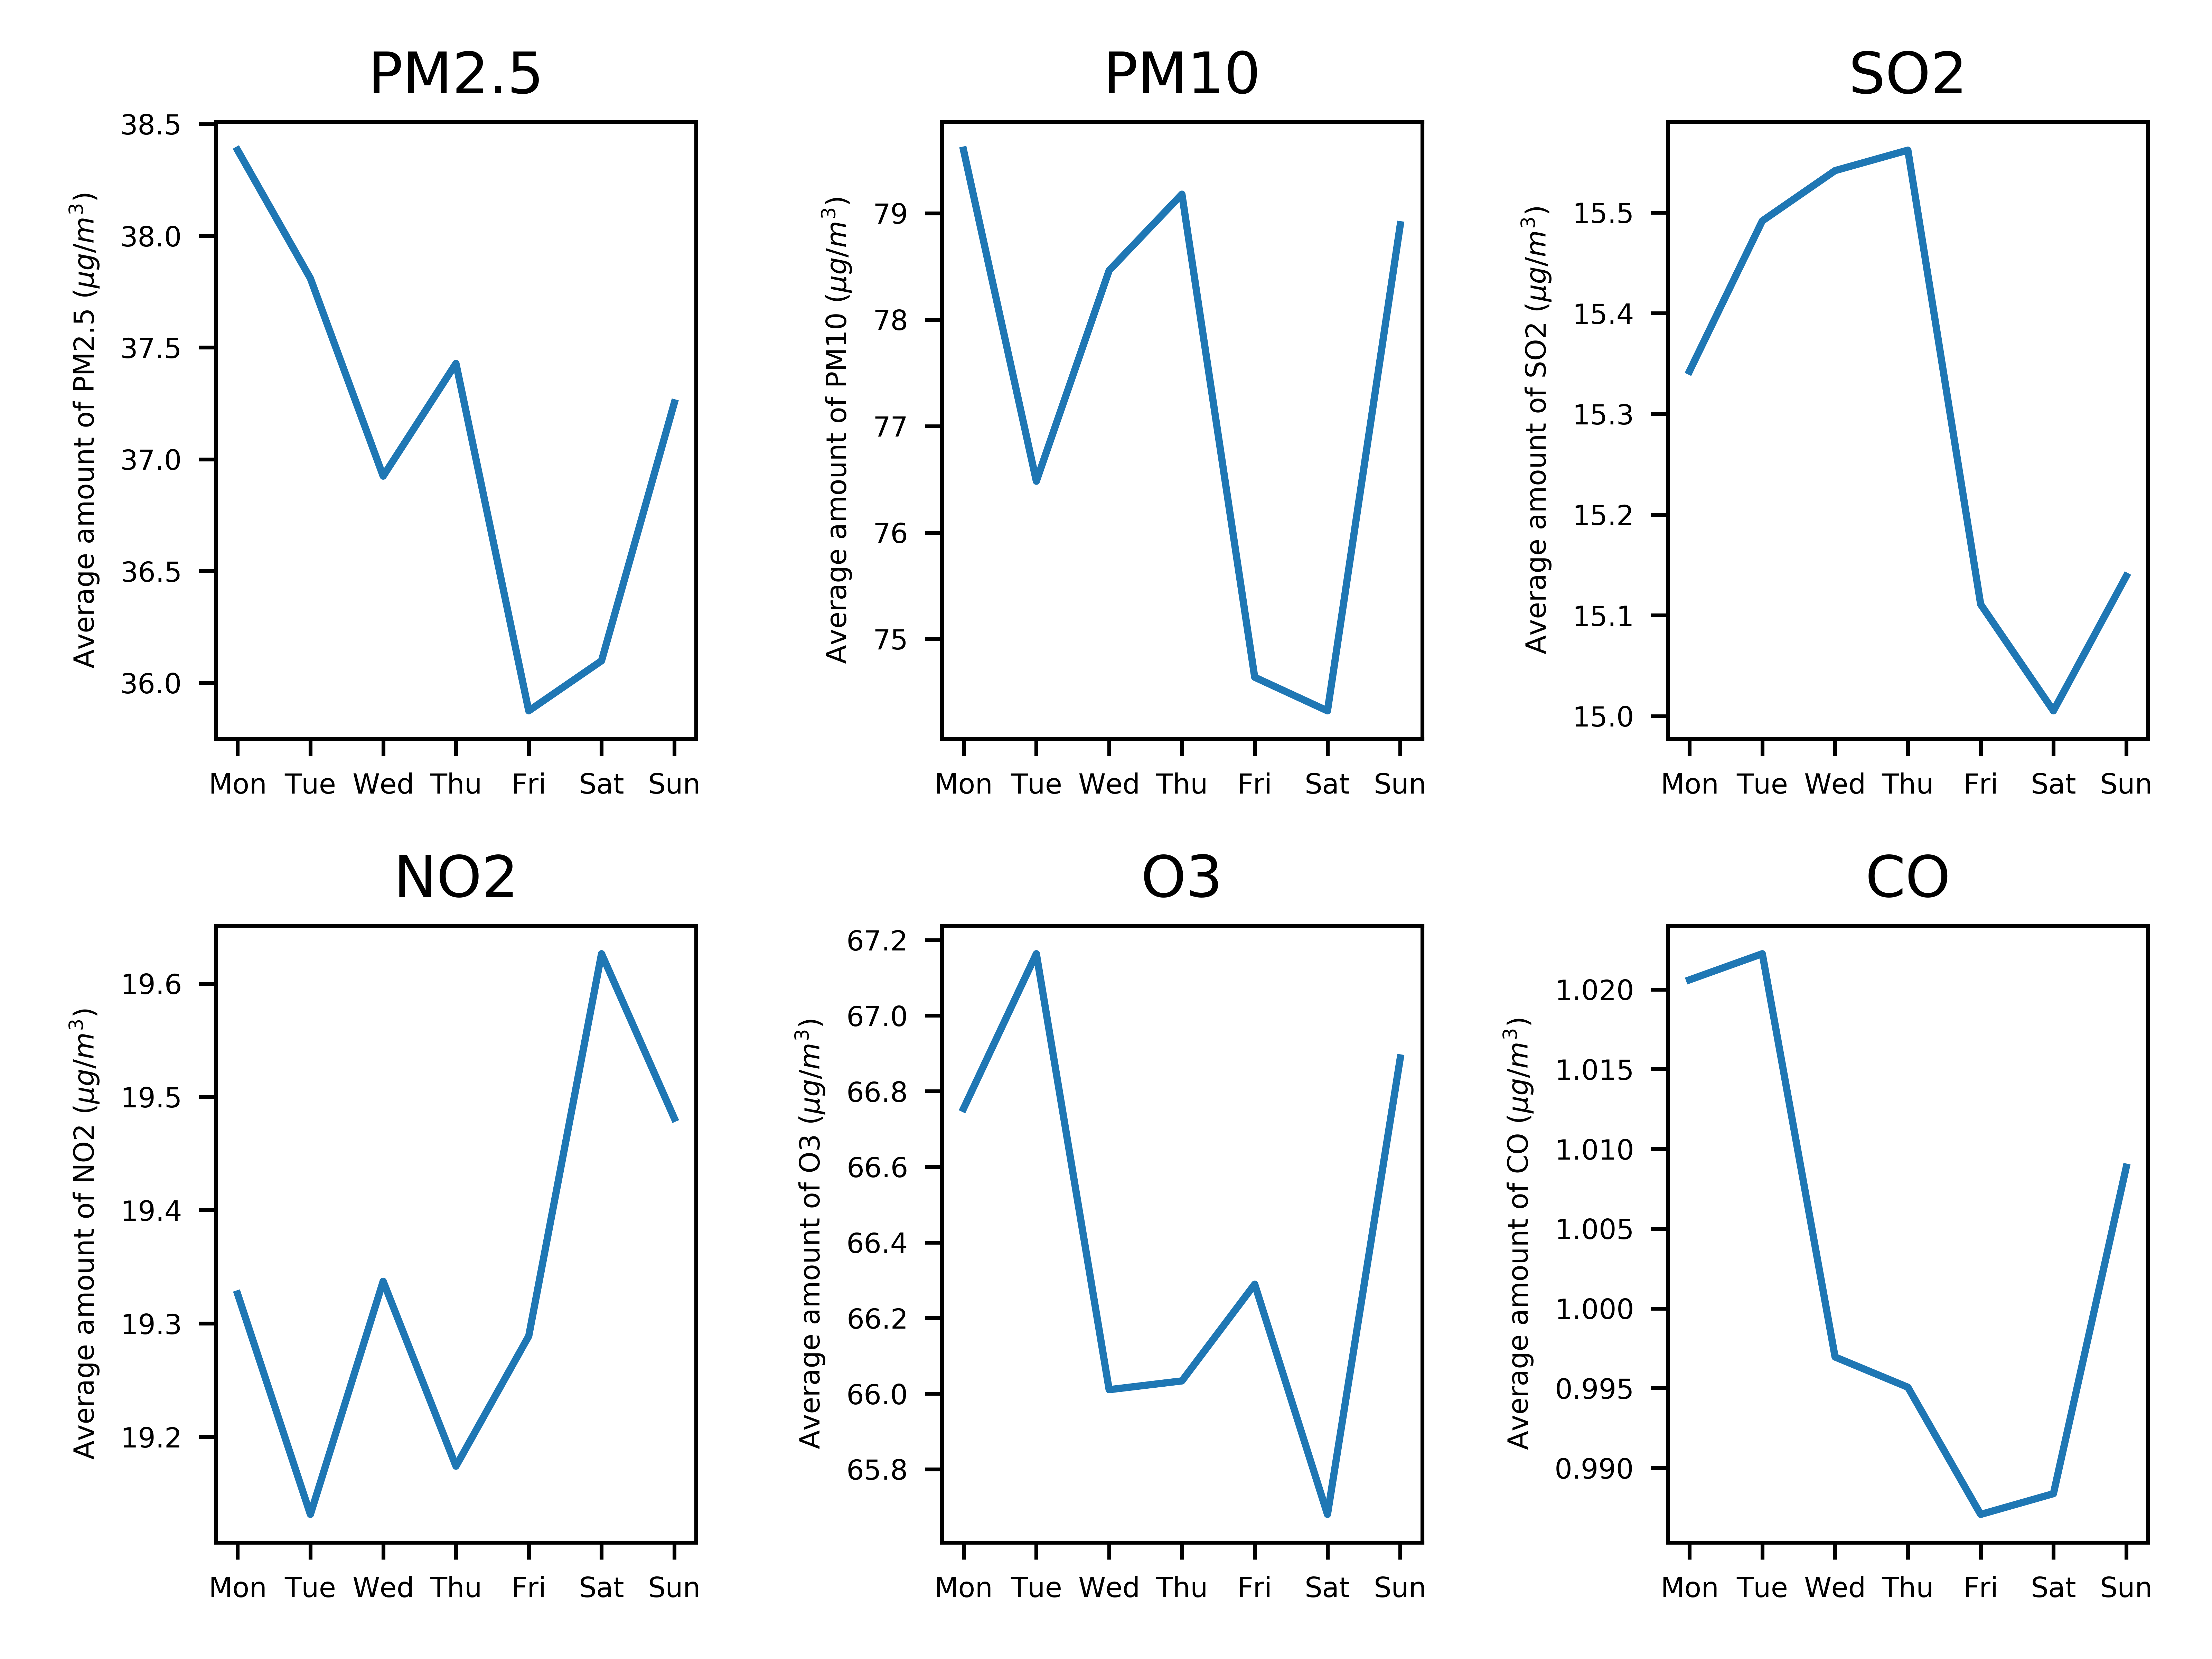
\includegraphics[width = 8.5cm]{weekavg_pltn.png}
  \caption{Weekly average concentration of pollutants}
  \label{figure:3}
\end{figure}

The figures shows the change curves of average daily concentration from Monday to Sunday. However, the curves seem zigzag and irregular, which can not reflect any regularities of weekly concentration changes. That means that the regularity of human weekly activities is not shown in the concentration changes.

\begin{figure}[h]
  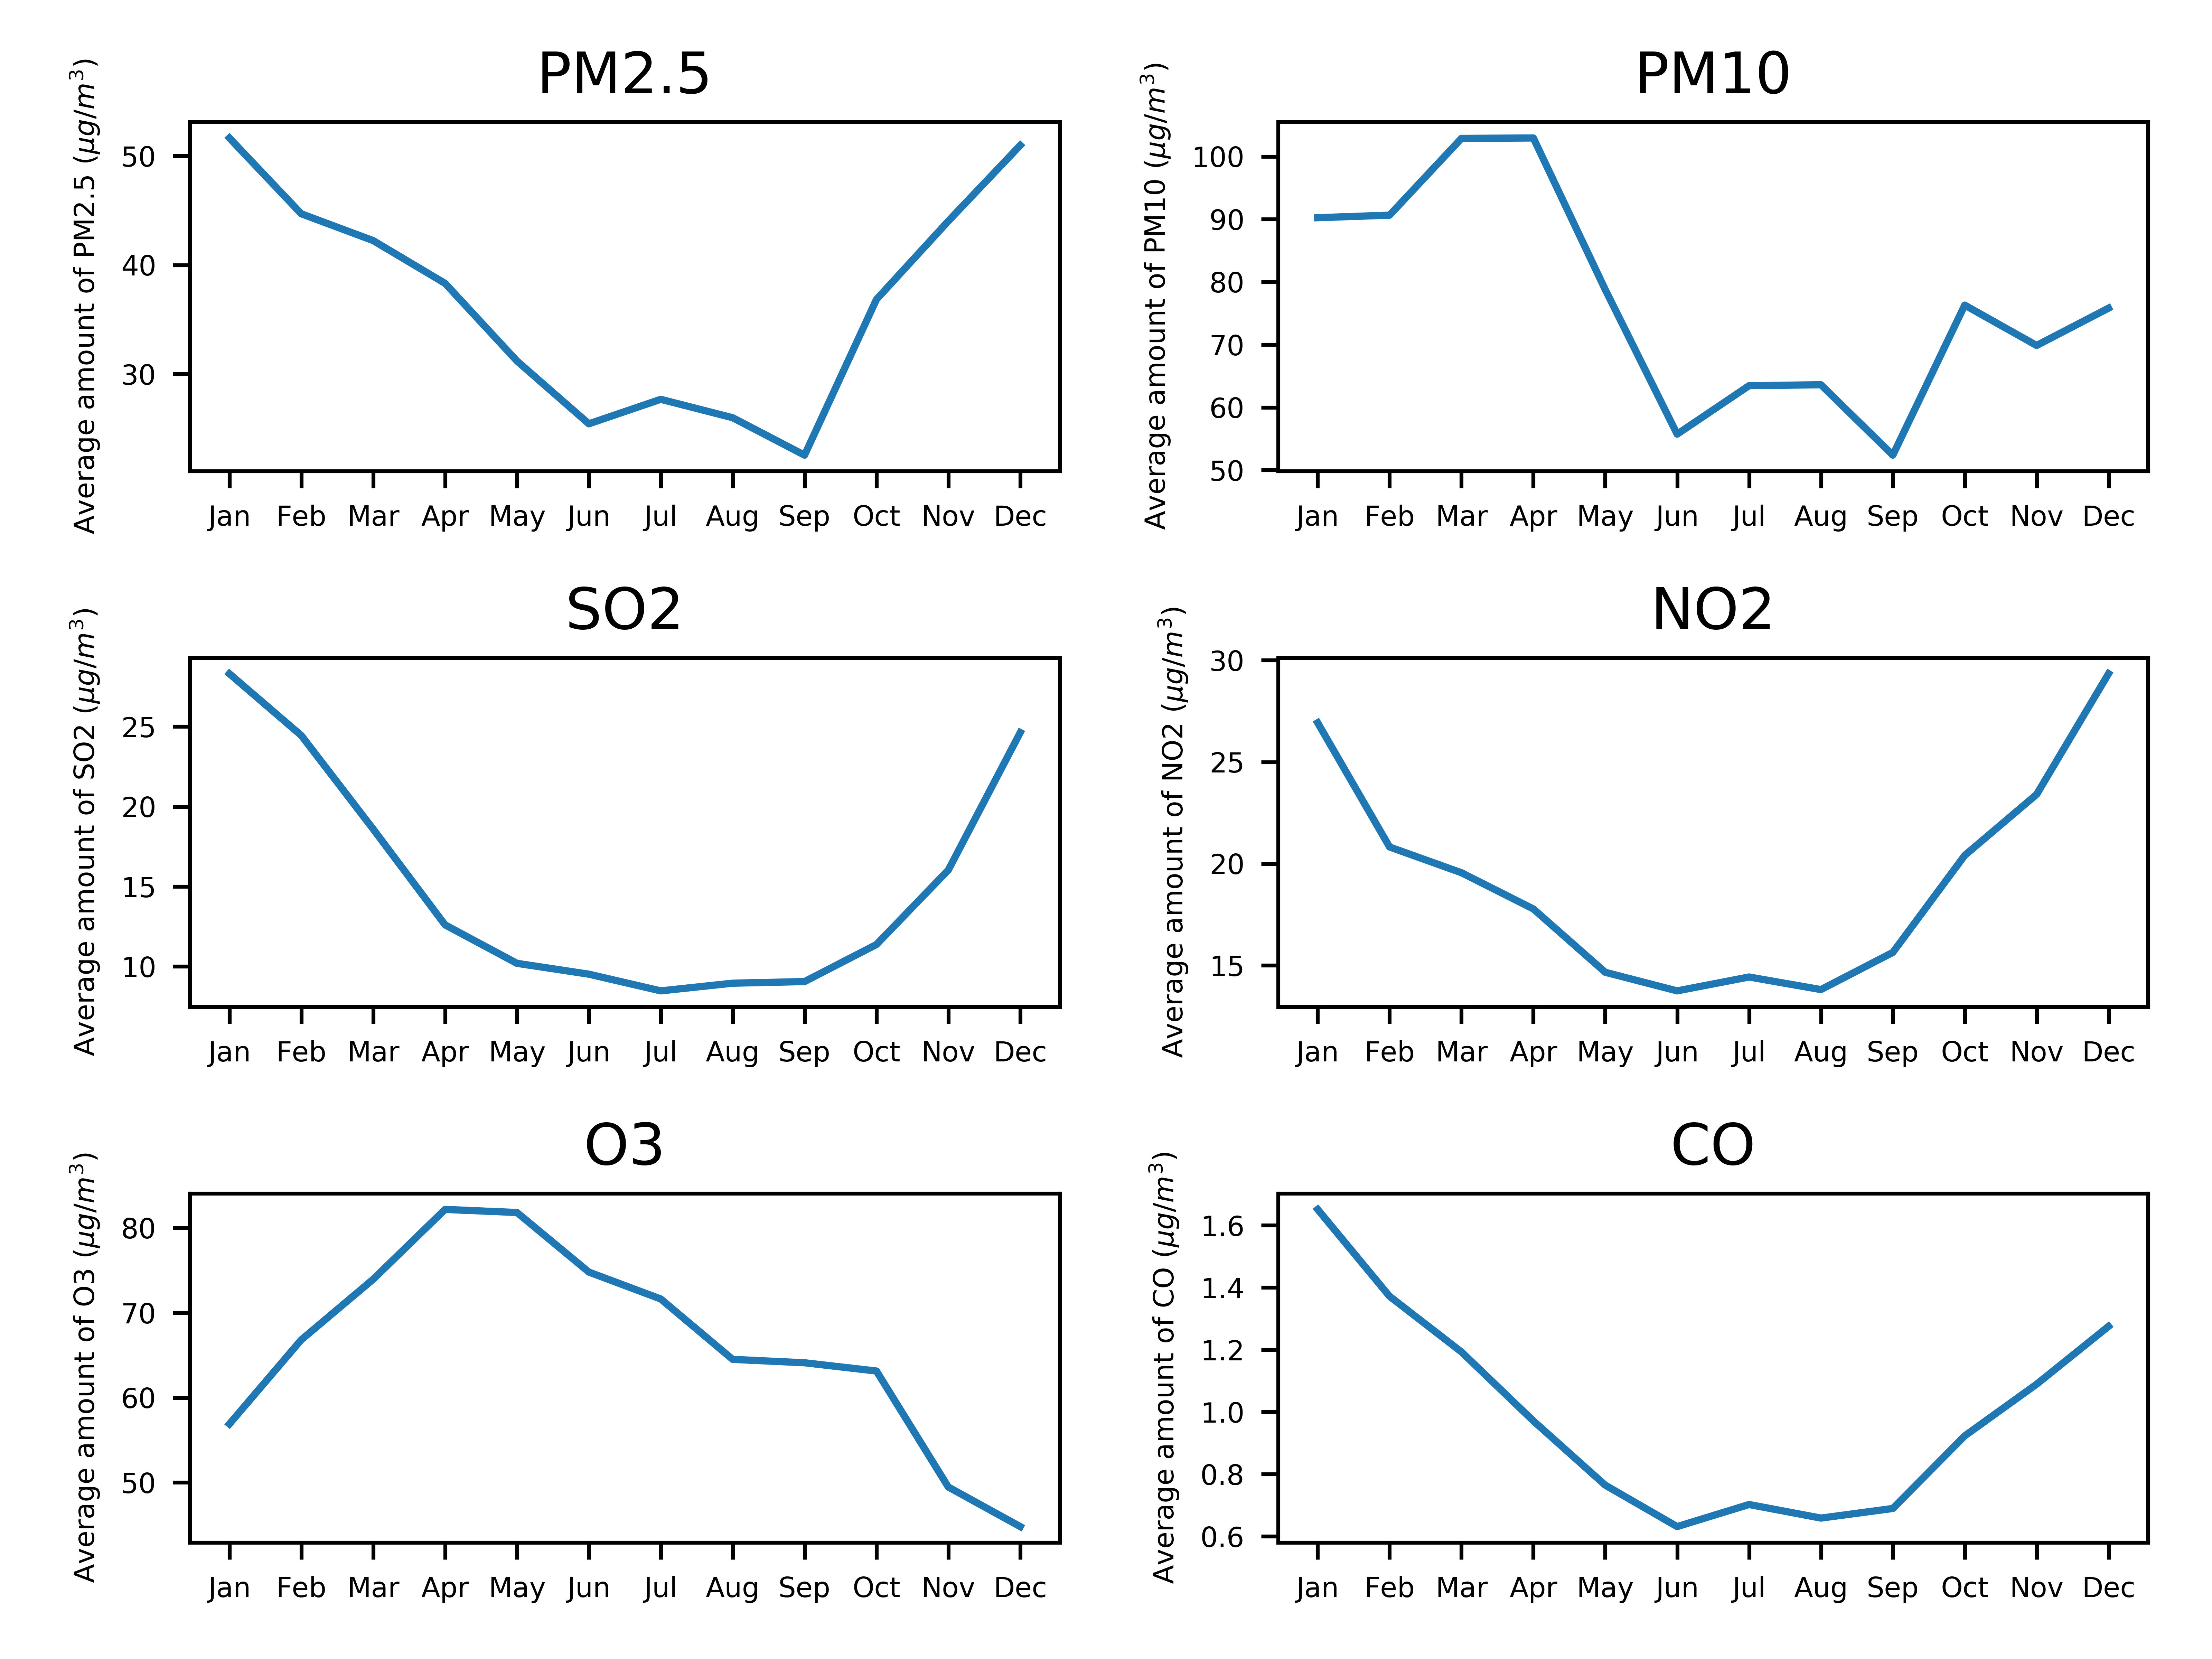
\includegraphics[width = 8.5cm]{monavg_pltn.png}
  \caption{Monthly average concentration of pollutants}
  \label{figure:4}
\end{figure}

The figures shows the change curves of average monthly concentration over the whole year. As it shows, the shape of concentration curves of PM$_{2.5}$, PM$_{10}$, SO$_{2}$, NO$_{2}$, and CO is like a letter U. The concentration decreases from January to June, keeps a low value from June to September, and increases from September to December. The curve of O$_{3}$ is special again. It is an inverted-U with a peak around April and May.

\subsection{Reason (TODO)}

\section{The Independence of Space Distribution and Time Distribution}

The regularities of space distribution and time distribution of pollutants have been concluded above. Another valuable topic to discussed is the independence of space distribution and time distribution. In other words, that is the space universality of time distribution and the time universality of space distribution. To simplify the analyse, AQI is used to represented the integrative concentration of six main air pollutants.

\begin{figure}[h]
  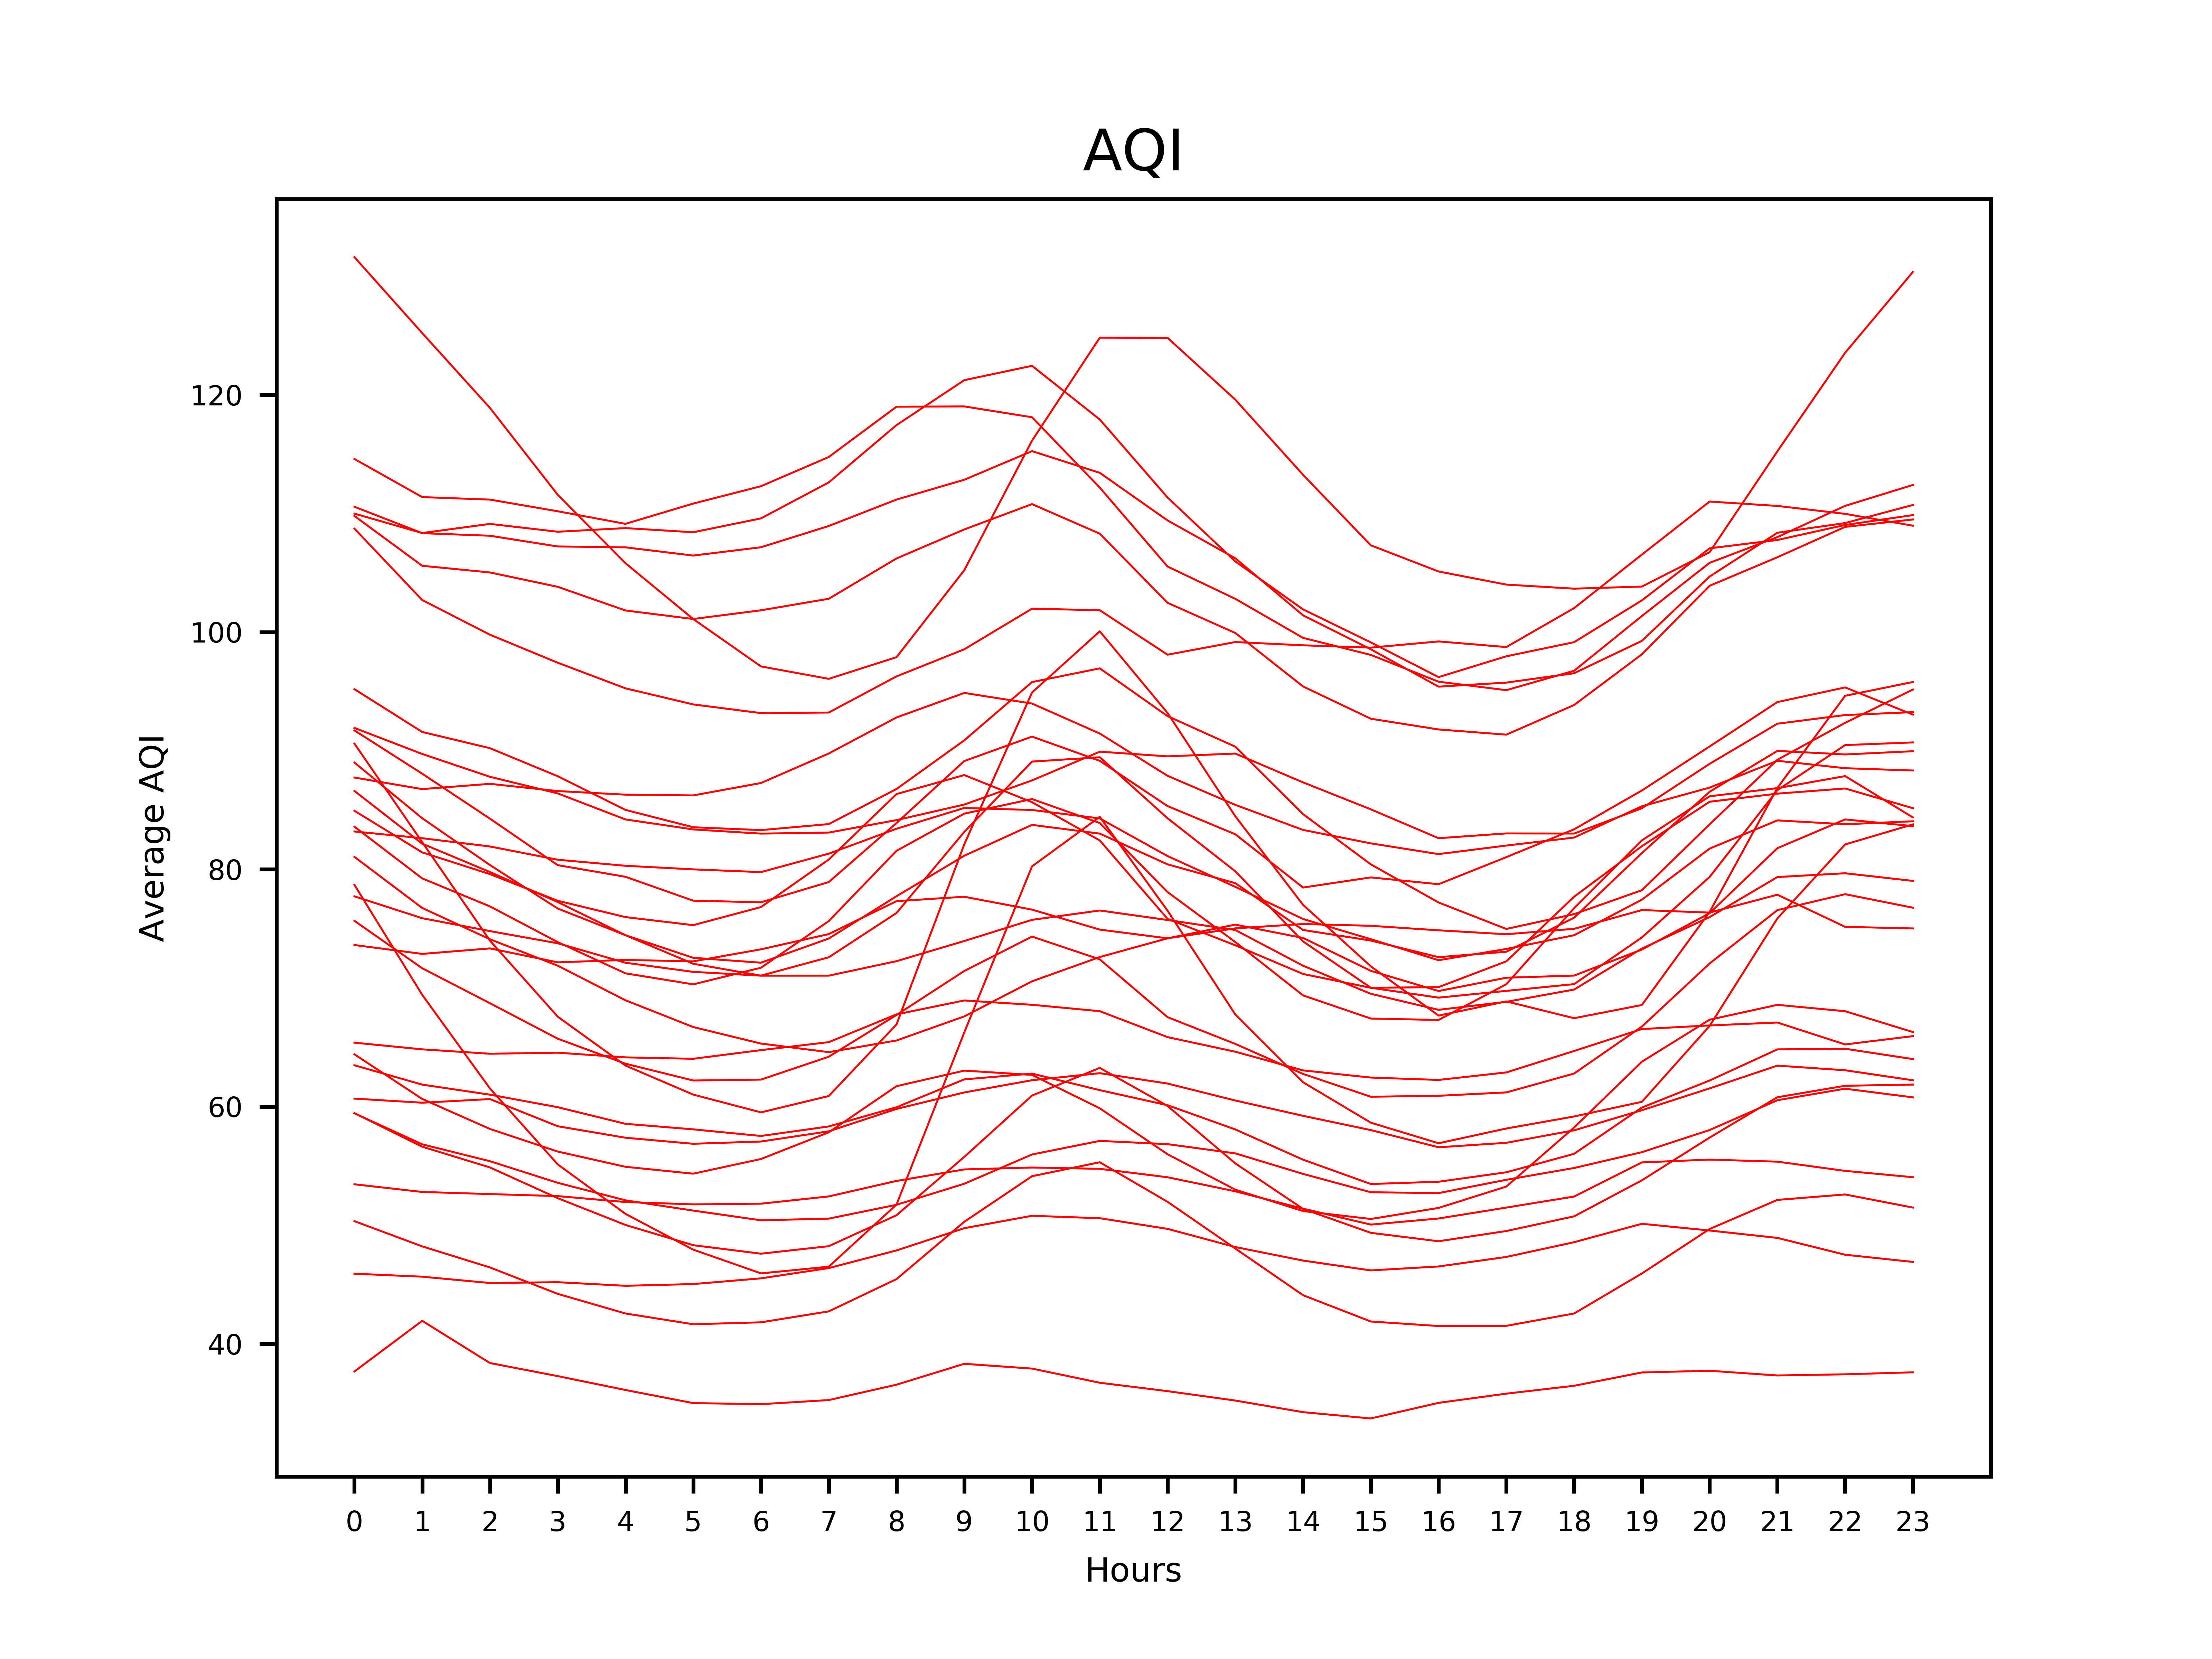
\includegraphics[width = 8.5cm]{dailyavg_pro_pltn.png}
  \caption{Daily average concentration of AQI for all provinces except Taiwan (lack of data)} 
  \label{figure:5}
\end{figure}

The figure analyses the change curves of average AQI over 24 hours for every province in China. The shape of curves in the figure are all similar, which shows that the regularity of daily distribution is general in all province in China. It is interesting that some provinces with low pollution have curves with little fluctuation. For example, the curve that represents Hainan, which is at the bottom of the figure, is nearly a horizontal line. This educes a reasonable educt that the regions with good air quailty have less changes of AQI.

\begin{figure}[h]
  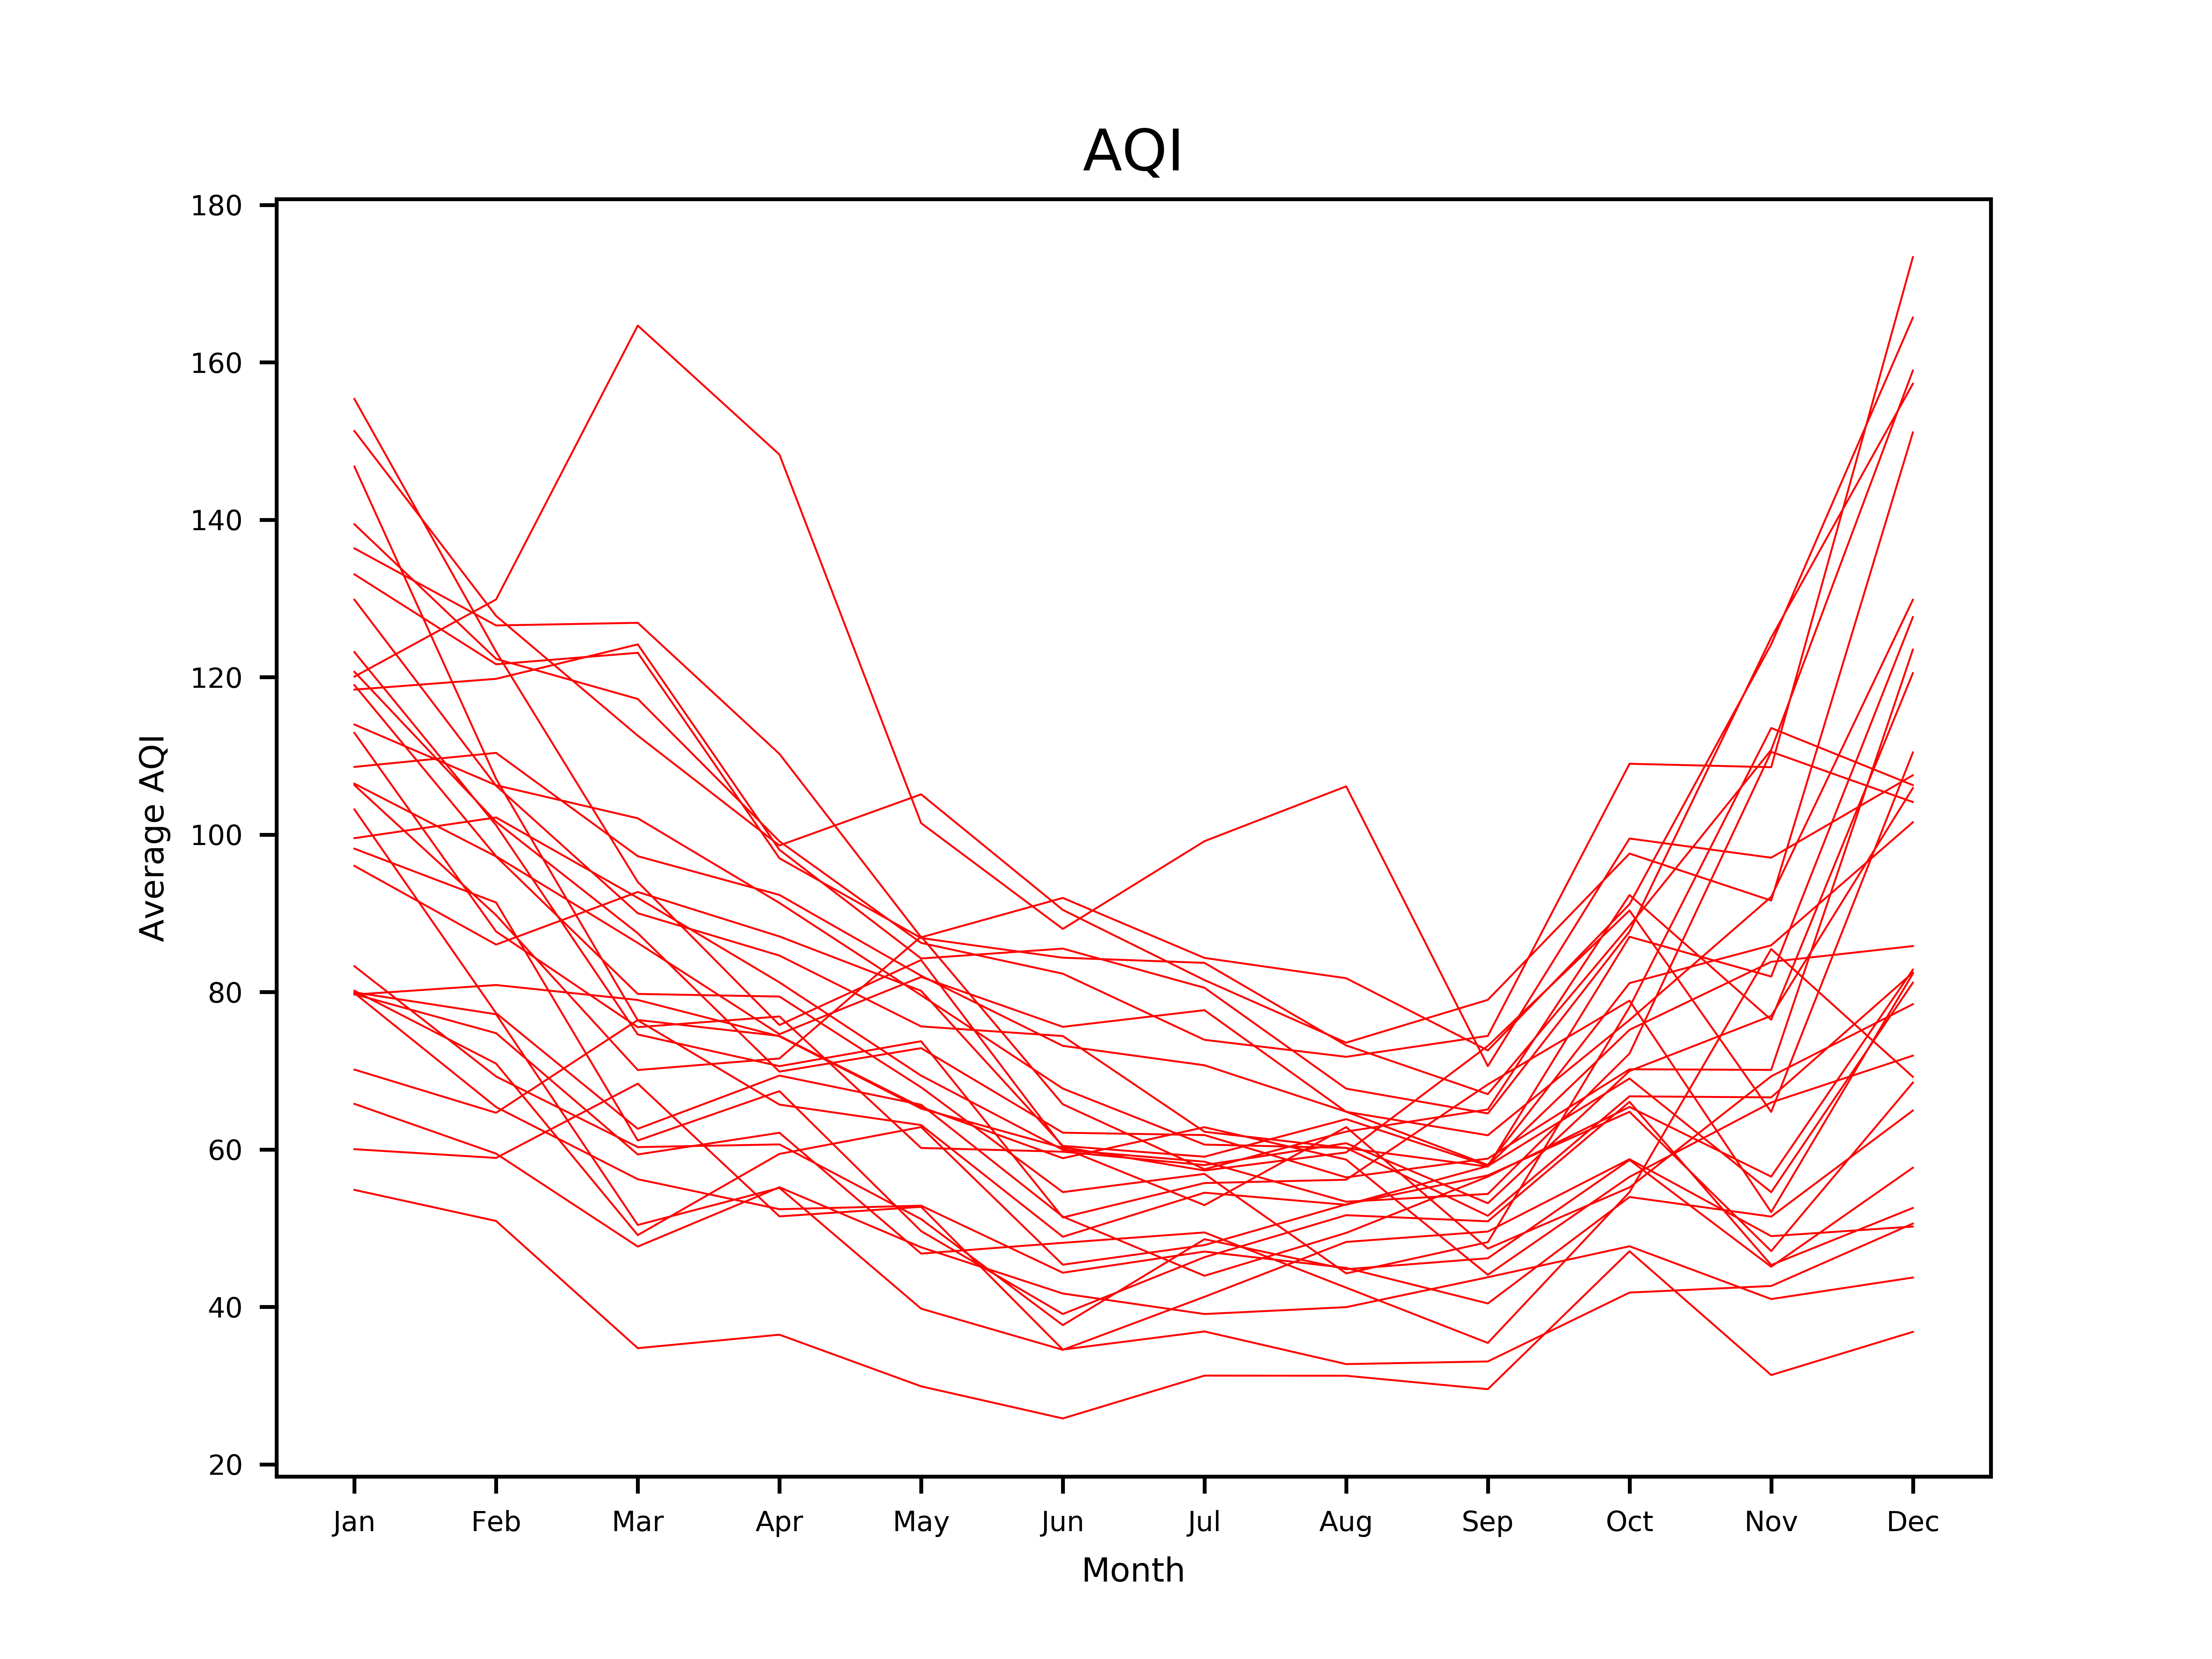
\includegraphics[width = 8.5cm]{monavg_pro_pltn.png}
  \caption{Monthly average concentration of AQI for all provinces except Taiwan (lack of data)} 
  \label{figure:6}
\end{figure}

The figure shows the change curves of monthly average AQI over the whole year for every province in China. It can be seen that all curves are roughly U-shaped, which conforms with the regularity summarized above and shows that the regularity is spacial general. Similar to the daily distribution, the conclusion that lower AQI is with less changes is also applied in this figure.

It can be found that the curve of Xinjiang, which is at the top of the figure, is the most special. A possible reason is the unique natural and geographical conditions in Xinjiang. Another interesting phenomenon is that the AQI increases quickly between September and October in many province, which means that this is a general phenomenon in China. Similar to the analyses for 2014 in former research, the reason may be some special pollution processes in October, which leads to the decline in air quality across China. However, it can not be proved by the data.

\begin{figure}[h]
  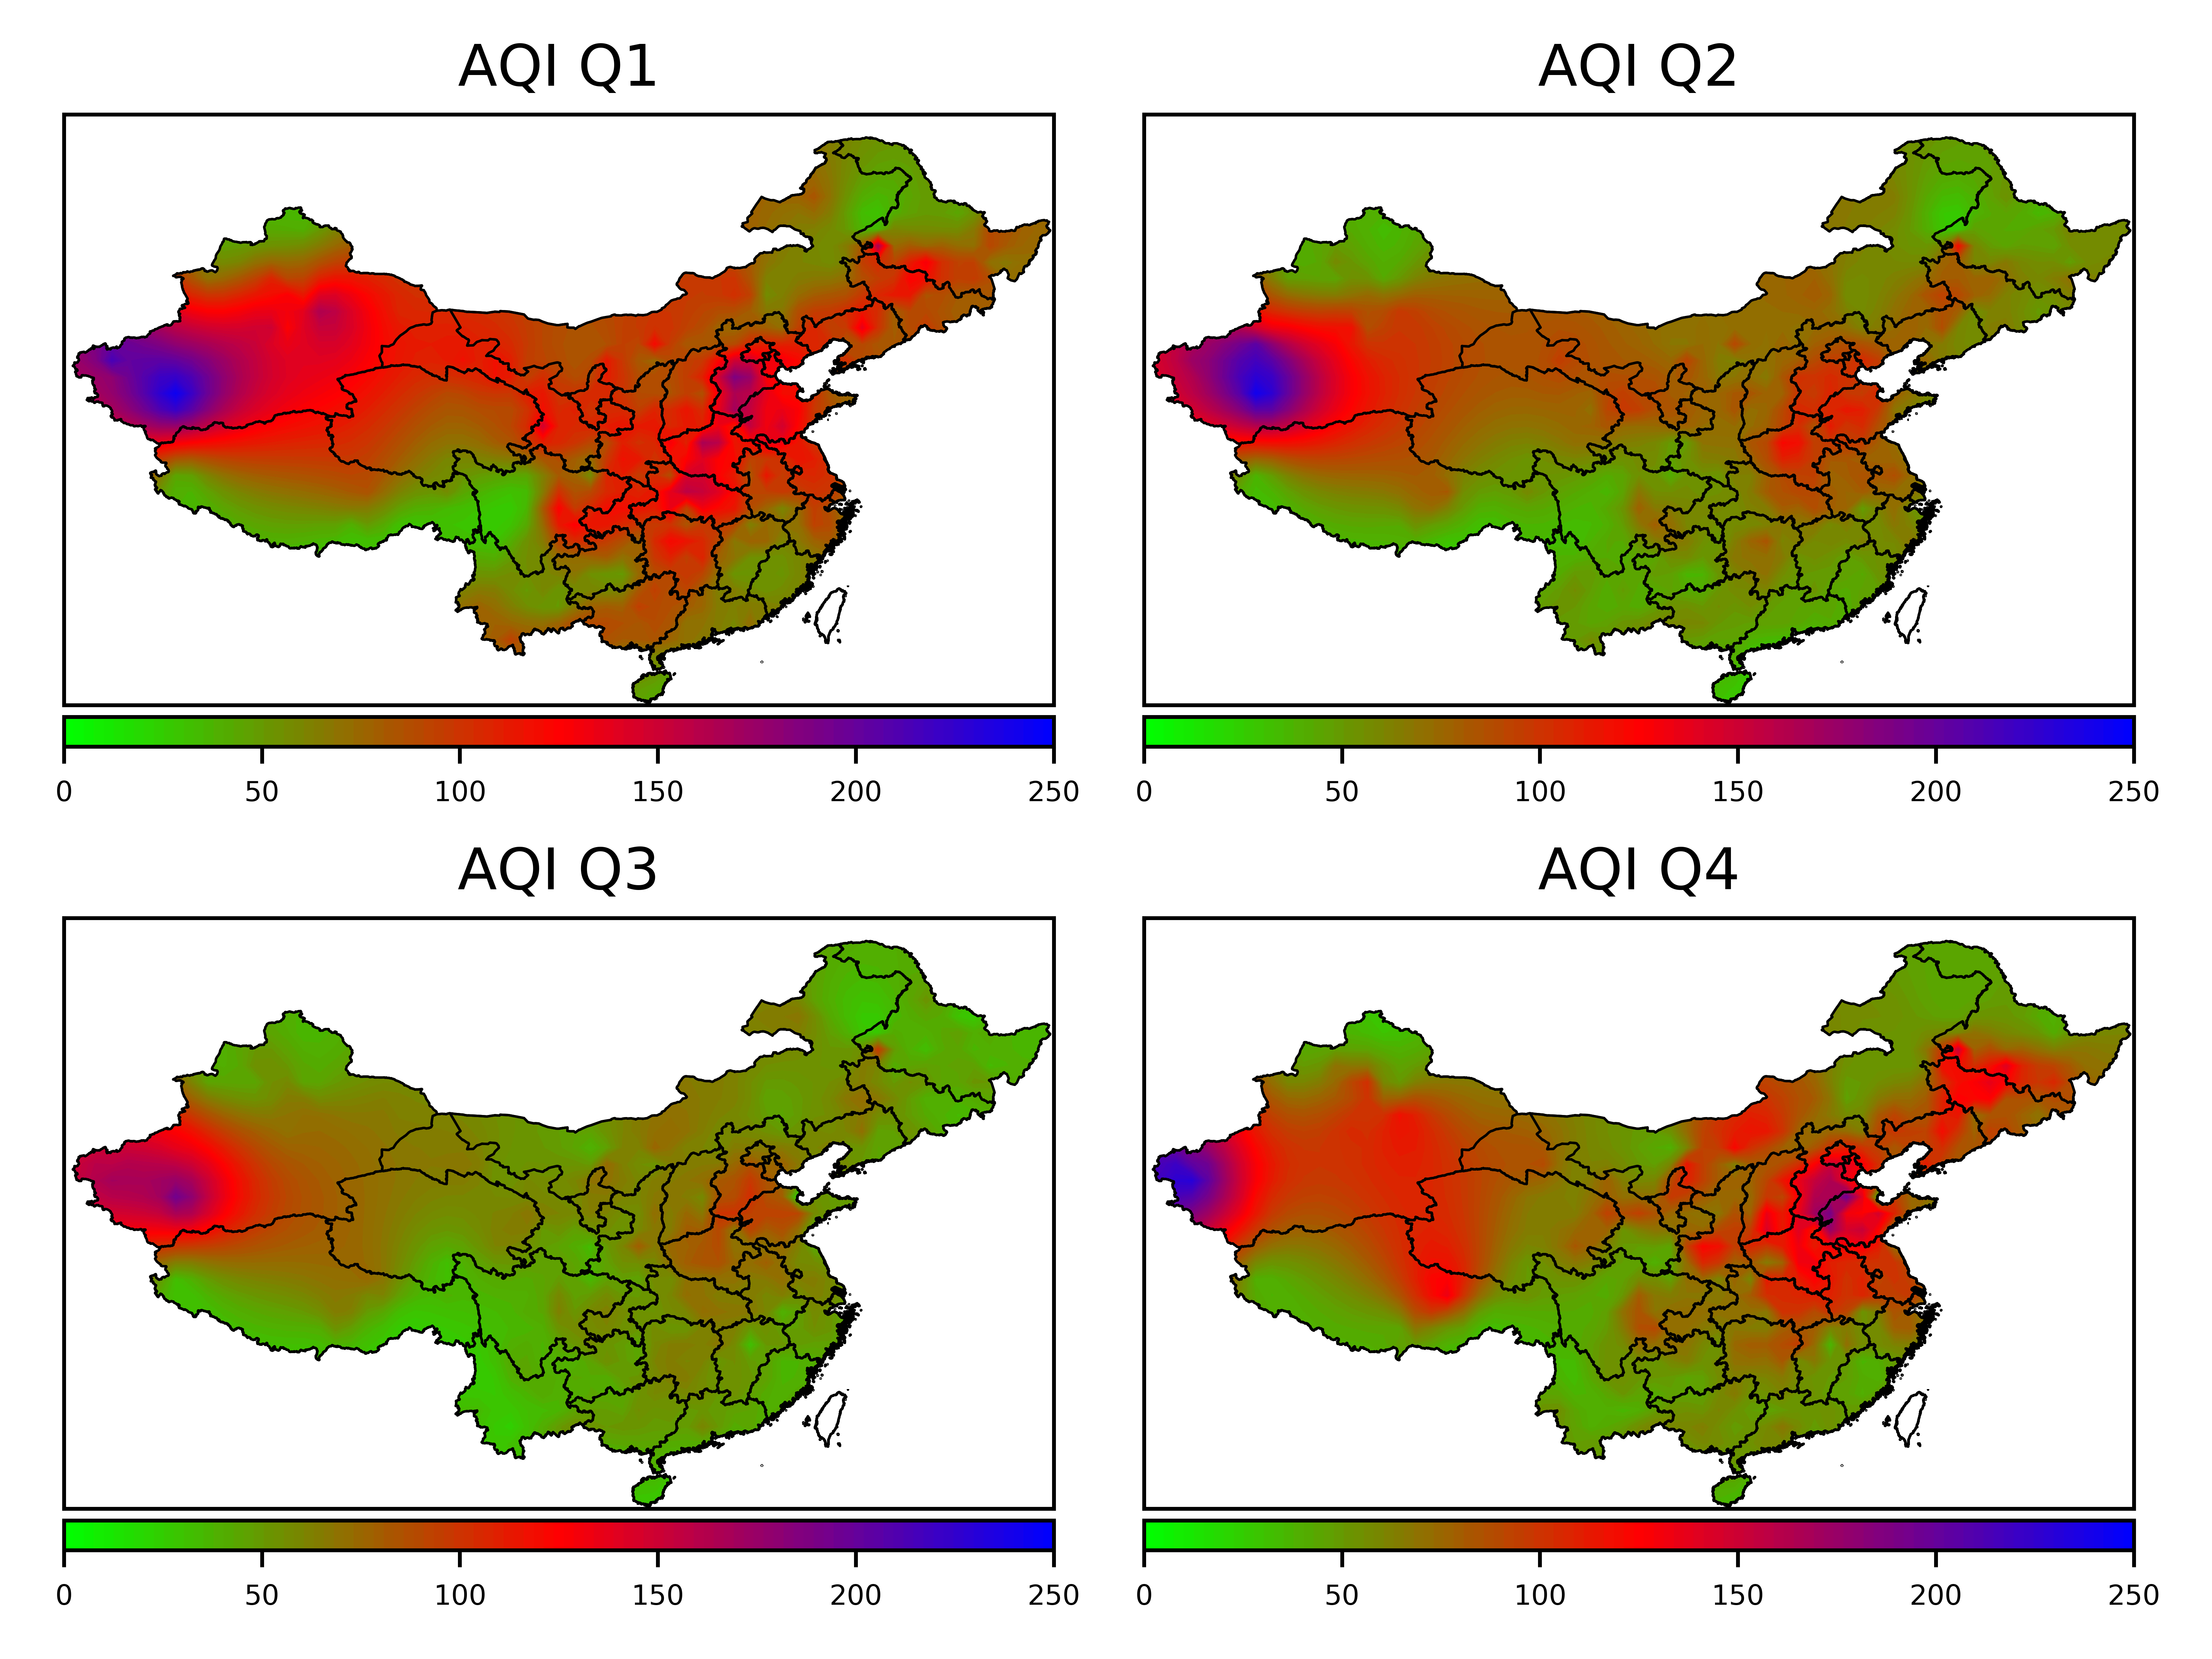
\includegraphics[width = 8.5cm]{AQI_season.png}
  \caption{Average AQI in 4 seasons}
  \label{figure:7}
\end{figure}

The figure is the space distribution of AQI in China in spring, summer, autumn, and winter. It can be found that the distribution does not change a lot in four season, which means that the space distribution is general in the whole year. The visible difference is the integral level of AQI, and the regularity has been discussed above. As the figure shows, the AQI in spring and winter is higher than that in summer and autumn, which matches the conclusion above. 

According to the discussion above, the independence of space distribution and time distribution of air pollutants has been verified preliminary.

\section{Comparison with Standard}

The space distribution and time distribution of air pollutants is discussed in detail above. However, the perniciousness of air pollutants can not be easily expressed by the concentration only without considering the standards.

The standards are different in different countries. In China, the latest ambient air quality standards is \textbf{GB 3095-2012}. In this part, the standards will be used to measure the effect of air pollutants on people.

\begin{table*}
  \begin{tabular}{c|cccc}
    \bf{Province} & \bf{PM2.5} & \bf{PM10} & \bf{SO2} & \bf{NO2} \\\hline
    \csvreader[head to column names]{./csv/provincial_annual_pollutant.csv}{}{\\\csvcoli & \csvcolii & \csvcoliii & \csvcoliv & \csvcolv}
  \end{tabular}
  \centering
  \caption{Annually average concentration of pollutants in all provinces}
  \label{table:2}
\end{table*}

The sheet shows the annual average concentration of PM$_{2.5}$, PM$_{10}$, SO$_{2}$, and NO$_{2}$ for every province. CO and O$_{3}$ are not considered because there are no annual average concentration standards for CO and O$_{3}$ in \textbf{GB 3095-2012}. It is not difficult to find that the concentrations of SO$_{2}$ and NO$_{2}$ satisfy secondary standards nearly in every province. However, there are only 7 and 10 provinces with concentration that satisfies secondary standard of PM$_{2.5}$ and PM$_{10}$ respectively. which is much worse than the situation of PM$_{2.5}$ and PM$_{10}$. That means the main pollutants that effect people are PM$_{2.5}$ and PM$_{10}$.

A important value to measure the air quality is AQI. According to the computing method of AQI, AQI depends on the concentration of a pollutant that makes the most serious pollution. AQI is between 0 and 50 when all kinds of pollutants reach primary standard and is between 0 and 100 when all kinds of pollutants reach secondary standard.

%%

The table counts the number of days with AQI falling in six intervals, which represent different air quality level, for every province. It also shows the total number of days for all province together. It can be found that the number of days with AQI at level 1 and level 2 is more than eighty percent, and that the number of days with AQI at level 1 is more than quarter. Thirteen provinces had more than ninety percent of days with AQI no more than 100. That means the overall air quality in 2015 was not bad. However, days with AQI at level 5 and level 6 exist, which means that there is some days with very serious pollution in some regions, such as Beijing-Tianjin-Hebei Region.


\begin{table*}[t]
  \begin{tabular}{c|cccccccc}
    \bf{Province} & \bf{0-50} & \bf{51-100} & \bf{101-150} & \bf{151-200} & \bf{201-300} & \bf{301-500} & \bf{Passing Rate($\mathbf{\leq 50}$)} & \bf{Passing Rate($\mathbf{\leq 100}$)} \\\hline
    \csvreader[head to column names]{./csv/valid_days.csv}{}{\\\csvcoli & \csvcolii & \csvcoliii & \csvcoliv & \csvcolv & \csvcolvi & \csvcolvii & \csvcolviii & \csvcolix}
  \end{tabular}
  \centering
  \caption{Days of AQI on different level in all provinces}
  \label{table:3}
\end{table*}

\end{document}

%%% Local Variables:
%%% mode: latex
%%% TeX-master: t
%%% End:
